\documentclass[12pt, twoside]{article}
\usepackage[letterpaper, margin=1in, headsep=0.5in]{geometry}
\usepackage[english]{babel}
\usepackage[utf8]{inputenc}
\usepackage{amsmath}
\usepackage{amsfonts}
\usepackage{amssymb}
\usepackage{tikz}
%\usetikzlibrary{quotes, angles}

\usepackage{graphicx}
\usepackage{enumitem}
\usepackage{multicol}

\usepackage{fancyhdr}
\pagestyle{fancy}
\fancyhf{}
\renewcommand{\headrulewidth}{0pt} % disable the underline of the header

\fancyhead[RE]{\thepage}
\fancyhead[RO]{\thepage \\ Name: \hspace{3cm}}
\fancyhead[L]{BECA / Dr. Huson / Geometry\\* 22 May 2019}

\begin{document}
\subsubsection*{11-3 Do Now: Using slope to prove theorems}
  \begin{enumerate}

  \item Given parallelogram $ABCD$ with $m\angle A=65^\circ$, $AB=4.5$, and $BC=7$. Find the value of each angle measure or side length.
    \begin{enumerate}
      \item $m\angle B=$\vspace{0.5cm}
      \item $m\angle C=$\vspace{0.5cm}
      \item $m\angle D=$\vspace{0.5cm}
      \item $CD=$ \vspace{0.5cm}
      \item $AD=$ \vspace{0.5cm}
    \end{enumerate}

  \item Three of the vertices of the parallelogram $ABCD$ are given: $A(1, 1)$, $B(8,2)$, $C(6, 6)$. Determine and state the coordinates of the fourth vertex, $D$, and mark and label it on the grid below. Draw the sides of the parallelogram.
    \begin{center}
      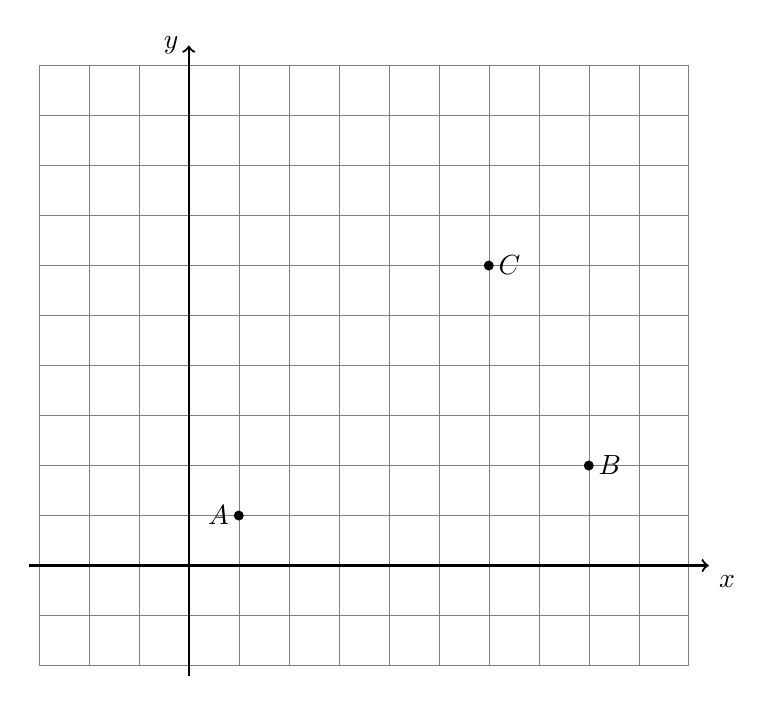
\begin{tikzpicture}[scale=.635]
        \draw [help lines] (-3,-2) grid (10,10);
        \draw [thick, ->] (-3.2,0) -- (10.4,0) node [below right] {$x$};
        \draw [thick, ->] (0,-2.2)--(0,10.4) node [left] {$y$};
        \fill (1,1) circle[radius=0.1cm] node[left]{$A$};
        \fill (8,2) circle[radius=0.1cm] node[right]{$B$};
        \fill (6,6) circle[radius=0.1cm] node[right]{$C$};
      \end{tikzpicture}
    \end{center}

\newpage

  \item Draw quadrilateral $ABCD$ with vertices $A(-2, 2)$, $B(6,0)$, $C(8,4)$, and $D(0,6)$ on the grid below. Prove that $ABCD$ is a parallelogram by using slopes to show $\overline{AB} || \overline{CD}$ and $\overline{AD} || \overline{BC}$. \\[0.5cm]
  Be sure to state that $m_{\overline{AB}}=m_{\overline{CD}}$ and $m_{\overline{AD}}=m_{\overline{BC}}$. Finish with a concluding statement.\\[1cm]
    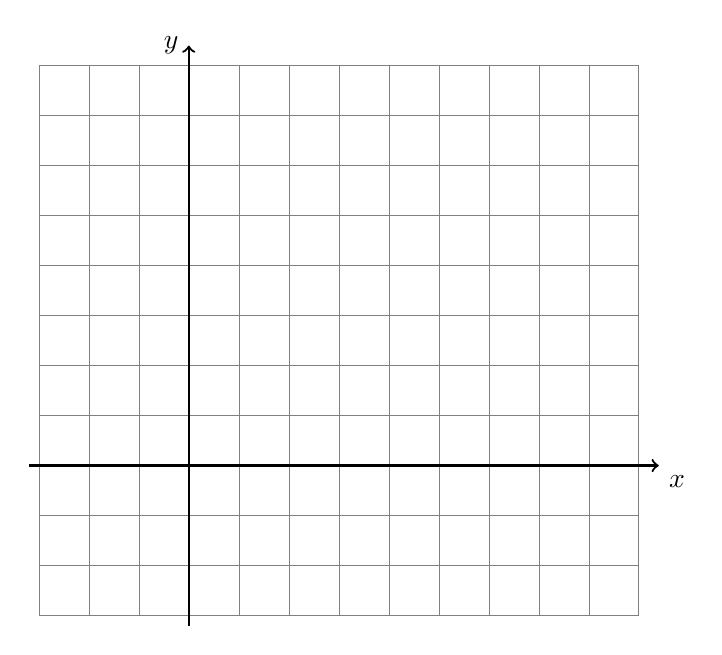
\begin{tikzpicture}[scale=.635]
      \draw [help lines] (-3,-3) grid (9,8);
      \draw [thick, ->] (-3.2,0) -- (9.4,0) node [below right] {$x$};
      \draw [thick, ->] (0,-3.2)--(0,8.4) node [left] {$y$};
    \end{tikzpicture}

\end{enumerate}

\end{document}
